\scanpage{133}
\mspage{15}
to $t$ and letting $t_1,\ldots,t_d$ be the unique elements in $k[[x_2,\ldots,x_n]]$ and $\deleted{t}\deleted{\unsure{t}}\inserted{\delta}$ \inserted{to} be the unique unit\deleted{$\unsure{t}$} in $R$ such that $\deleted{t=t'\unsure{t}}\inserted{t=t'\delta}$ where $t'=x_1^d+t_1x_1^{d-1}+\cdots+t_d$, we have that $t'$ divides $z$ in $k[[x_2,\ldots,x_n]][x_1]$.
\margin{Greek letter small ``delta''}
\margin{\figure{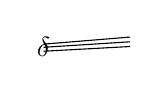
\begin{tikzpicture}\node at(0,0){\deleted{$\unsure{\delta}$}};\draw(0,.03)--(1.1,.12);\draw(0,-.01)--(1.1,.06);\draw(0,-.06)--(1.1,0);\end{tikzpicture}}}
Finally if $e$ is a non-zero element of $R$ and $u_1,\ldots,u_n$ is a basis of $M$ and either $k$ is infinite or $\lambda_R(e)\leq2=n$ then there exist elements $a_{ij}$ in $k$ such that letting $v_i=\sum a_{ij}u_j$ we have that $v_1,\ldots,v_n$ is a basis of $M$ such that the line $v_2=\cdots=v_n=0$ is non-tangential to $e$.

\uline{Proof}. We have $\Lambda(y)=cx_1^b+cf_1(x_2,\ldots,x_n)x_1^{b-1}+\cdots+cf_b(x_2,\ldots,x_n)$ where $0\ne c\in k$ and $f_i(X_1,\ldots,X_n)$ is either zero or is a form of degree $i$ in $k[X_2,\ldots,X_n]$. Therefore $y\notin(x_2,\ldots,x_n)R$ and hence $(y,x_2,\ldots,x_n)$ is primary for $M$. Let $S=k[[x_2,\ldots,x_n]]$, $N=(x_2,\ldots,x_n)S$ and let $\deleted{t}\inserted{\tau}$ be the canonical homomorphism of $R$ onto $R/yR$. Then $\deleted{tN}\inserted{\tau N}$ is primary for $\deleted{t}\inserted{\tau}M=(\deleted{t}\inserted{\tau}x_1,\ldots,\deleted{t}\inserted{\tau}x_n)(\deleted{t}\inserted{\tau}R)$.
\margin{Greek letter small ``tau''}
In proving the existence of $y_1,\ldots,y_b,\eta$, without loss of generality we can assume that $y$ is irreducible in $R$, for in the general case we can apply the result to each irreducible factor of $y$ and multiply out the corresponding powers of the ensuing polynomials and we would get the required polynomial for $y$; also if $y$ is divisible by $x_1$ in $R$ then since we are assuming that $y$ is irreducible in $R$ we can take $y'=x_1$; so now assume that $y$ is irreducible in $R$ and is not divisible by $x_1$. Then $\deleted{t}\inserted{\tau}N$ is primary for
\mspage{132}
